\documentclass[10pt]{IEEEtran}
\pdfoutput=1

\usepackage{graphicx}
\usepackage{hyperref}
\usepackage[utf8]{inputenc}
\usepackage{listings}
\usepackage[table]{xcolor}
\usepackage{pdfpages}
\usepackage{algpseudocode}
\usepackage{natbib}
\usepackage{tikz}
\usetikzlibrary{shapes,shadows,arrows}

%style to be used on block diagrams
\tikzstyle{block} = [draw,rectangle, fill=white]
\tikzstyle{line} = [draw,thick]
\tikzstyle{arrowLine} = [draw,-stealth,thick]

%style to be used on flow charts diagrams
\tikzstyle{startstop} = [rectangle, rounded corners, minimum width=2.5cm,
minimum height=0.75cm,text centered, draw=black,fill=red!30]
\tikzstyle{io} = [trapezium, trapezium left angle=70,trapezium right angle=110,
minimum width=2.5cm,minimum height=0.75cm,text centered, draw=black,fill=blue!30]
\tikzstyle{process} = [rectangle, minimum width=2.25cm, minimum height=0.75cm, text centered, draw=black, fill=orange!30]
\tikzstyle{decision} = [diamond, minimum width=2cm, minimum height=0.5cm, 
text centered, draw=black,fill=green!30]
\tikzstyle{flowArrow} = [thick,->,->=stealth]


\hypersetup{colorlinks=true,citecolor=[rgb]{0,0.0,0}}


\title{Data mining with python: \\Automated FOREX trading}
\author{
	Kevin Voss Sjøbeck(s103451)\\
	\and
	Benjamin Maksuti(s103449)\\
	\and
	Anders Wessberg(s103477)
}


\begin{document}
\maketitle

\begin{abstract}
This project will utilize the oandapy API to get realtime data from the currency market to analyze, as well as enter and exit trades on based on the analytics. In the analytics we are going to use a short and a long moving averages, furthermore we are going to use MCAD as an extra precaution before we enter trades and use recovery zones to prevent losses on the account
\end{abstract}

\section{Introduction}
Here will be written an introduction


\section{Analysis}

\subsection{Getting data}
We obtain all the financial data of the financial instrument EUR vs USD on a 5 minute timeframe from oanda using their REST API for python. From oanda API we get the financial charts of the last 7 years from 2007-10-24 to 2014-10-24. After obtaining the data, it is stored in json fileformat in a file called "fxdata.txt", this allows us to use this data will then be used both to form our hypothosis of forex trading on the EUR vs USD currency pair, as well as performing a trading simulation on this set of data. However in order for us to use the naive Bayes classifier, we need to have two dataset's and not just a single one. In our domain the one dataset needs to be the trades which gained profit, and the other set needs consist of the trades which lost. When we then have the possibility to analyze the data with different sets of features.\\
\\
The pseudo code of the random trading algorithm, where we will keep the orders for no more than 20 minutes:

\begin{center}
\begin{algorithmic}
\While{$streamFinancialData$}
	\State {$i = random(0,10)$}
	\If {$i = 0$}
    	\State {$openOrder(short)$}
	\ElsIf{$i = 1$}
    	\State $openOrder(long)$	    
	\EndIf
	\For{$order\: in\: orders$}	
		\If{$order.hasProfit()$}
			\State{$profitList.append(order)$}
			\State{$order.close()$}
		\ElsIf{$order.hasLoss()$}
			\State{$lossList.append(order)$}
			\State{$order.close()$}
		\ElsIf{$order.duration >= 4$}
			\State{$order.close()$}
		\Else
			\State{$order.duration += 1$}
		\EndIf
	\EndFor
\EndWhile
\State{$saveListToFile(profitList,"profit.txt")$}
\State{$saveListToFile(lossList,"loss.txt")$}
\end{algorithmic}
\end{center}

This algorithm should theoretically give us equally profitable trades in both the long and the short direction.

\subsection{Specific features}
To analyze the data we use a supervised classification learning algorithm, or to be more specific we use a naive Bayes classifier, the idea is to use a naive Bayes classifier on our financial data we gathered using our random algorithm. This isn't a new concept, in fact there are a couple of scientific articles on this already, as can be seen in the article by KAWABATA and TAKATA \cite{fxNaiveBayes}. We will train the classifier on some specific features, however we will only use 2-3 features per training round. The training will be made in two rounds and the features are the following
\begin{itemize}
	\item{CrossGraph(SMA(10,40))}
	\item{RSI(period=100)}
	\item{openBid(period=1)}
	\item{closeBid(period=1)}
	\item{volume(period=1)}
	\item{spread(period=1)}
	%\item{Parabolic SAR default settings (0.02, 0.2)}
	%\item{MACD default settings (fast=12, slow = 15, period=9)}
\end{itemize}

The first round of features, is using some of the most common technical indicators on the FX market, this should give a good indication if those are just famous for being simple or if you actually are able to earn profit using these indicators. The second round another of the more simple techniques that some of the professional FX traders should use according to chat on the different trading forums, this isn't really a technical indicator, it is much more a way to look at the market and only make a trade if the current price reaches a specific value. Our hypothosis is that the traders who use price actions looks only at the price, so that is exactly what we are going to do as well, and by giving the classifier the features of openBid, closeBid, volume, and spread we hope to achive the behaviour of a price action trader. On the third and last round of features, we searched the internet for a forex trading strategy on the EUR vs USD pair, to see how our strategies of the first two rounds of features compare to a random strategy you can find on the internet. The strategy we found consist of using SAR indicator as well as three different MACD indicators.

\begin{figure}
\begin{center}
	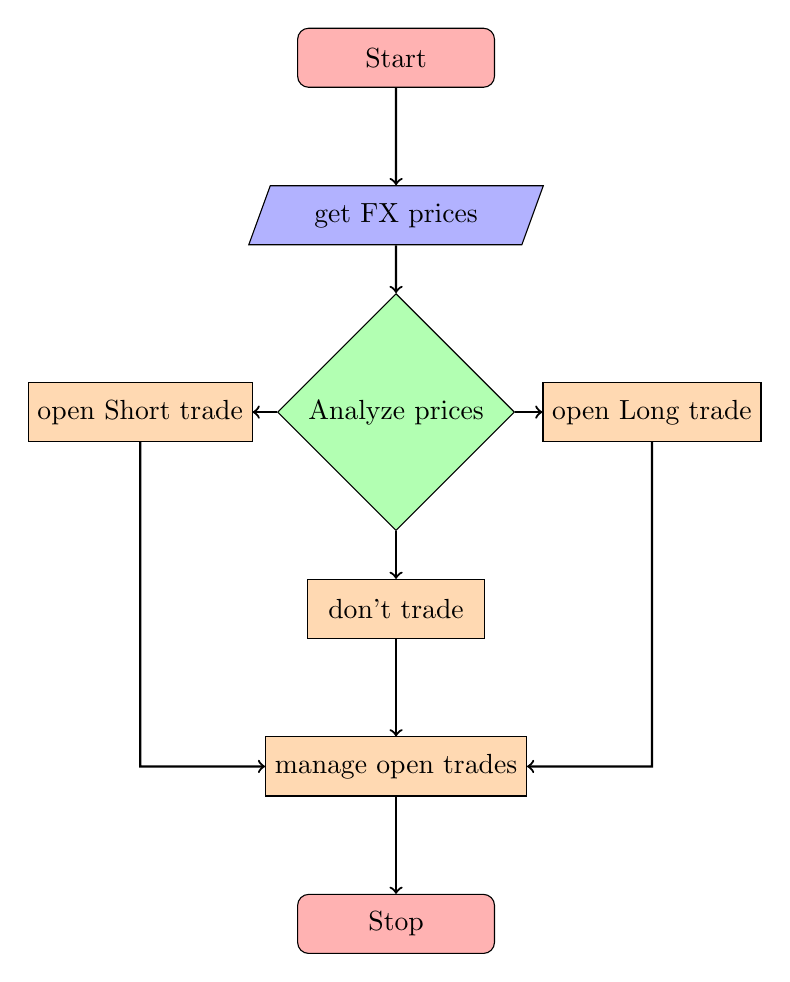
\begin{tikzpicture}[node distance=2cm]
		%blocks
		\node[startstop](start){Start};
		\node[io, below of=start](fx_price){get FX prices};
		\node[decision, below of=fx_price,yshift=-0.5cm](analyze){Analyze prices};	
		\node[process, right of=analyze, xshift=1.25cm](long){open Long trade};
		\node[process, left of=analyze, xshift=-1.25cm](short){open Short trade};
		\node[process, below of=analyze,yshift=-0.5cm](no_trade){don't trade};		
		\node[process, below of=no_trade](manage){manage open trades};				
		\node[startstop, below of=manage](stop){Stop};		
		
		%arrows			
		\draw[flowArrow](start)--(fx_price);
		\draw[flowArrow](fx_price)--(analyze);		
		\draw[flowArrow](analyze)--(long);		
		\draw[flowArrow](analyze)--(short);						
		\draw[flowArrow](analyze)--(no_trade);						
		\draw[flowArrow](no_trade)--(manage);
		\draw[flowArrow](short)--(-3.25,-9)--(manage);		
		\draw[flowArrow](long)--(3.25,-9)--(manage);		
		\draw[flowArrow](manage)--(stop);		
	\end{tikzpicture}
\end{center}
\caption{Flowchart of decision making}
\end{figure}


\section{Design}
Before we start trading, we need to start to train our classifier based on the feature set we would like to test. After the training is completed we can then start to trade based on our historical data. When the historical back testing is completed, the result of the trade is then shown on a graph, showing the balance of the account of a 5 minute interval. Here is a flow chart, showing how the flow of the forex data, and the decisions are being made.



\begin{figure}
\begin{center}
	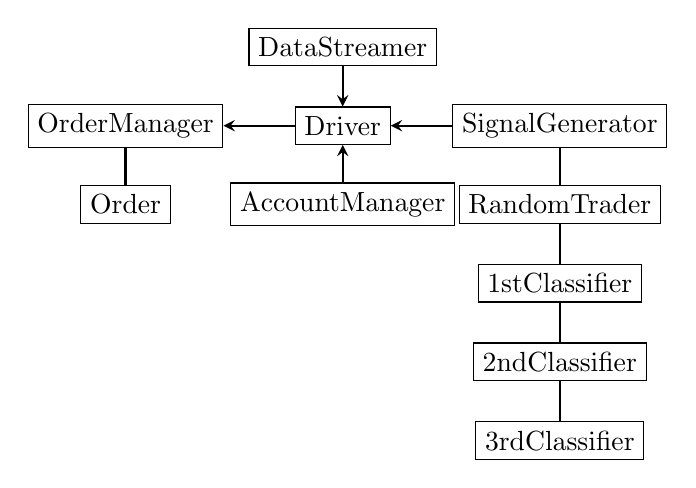
\begin{tikzpicture}
		\node[block](streamer){DataStreamer};
		\node[block,below of=streamer](driver){Driver};		
		\node[block,below of=driver](accountManager){AccountManager};				
		\node[block,left of=driver,xshift=-5em](orderManager){OrderManager};
		\node[block,below of=orderManager](order){Order};		
		\node[block,right of=driver,xshift=5em](signalGenerator){SignalGenerator};
		\node[block,below of=signalGenerator](random){RandomTrader};				
		\node[block,below of=random](1stClassifier){1stClassifier};		
		\node[block,below of=1stClassifier](2ndClassifier){2ndClassifier};		
		\node[block,below of=2ndClassifier](3rdClassifier){3rdClassifier};						
		%arrows
		\path[arrowLine](streamer)--(driver);		
		\path[arrowLine](accountManager)--(driver);				
		\path[arrowLine](driver)--(orderManager);
		\path[line](orderManager)--(order);
		\path[arrowLine](signalGenerator)--(driver);
		\path[line](signalGenerator)--(random);				
		\path[line](random)--(1stClassifier);		
		\path[line](1stClassifier)--(2ndClassifier);
		\path[line](2ndClassifier)--(3rdClassifier);				
	\end{tikzpicture}
\end{center}
\caption{Overview of Classes}
\end{figure}




\section{Implementation}
Here we explain about the program itself

\section{Test \& Results}

\subsection{Test}
All of the classifiers will be tested using both a sort term test, and a long term test, the short term test is from September 2014 to October 2014, stretching over 5000 times 5 minutes. The long term test is stretching from 24th of October 2007 to 24th of October 2014 corresponding to about 535.000(536.252) times 5 minutes.
All of the classifiers have been tested using a strategy with take profit, and stop losses of a risk of 1:2 meaning that for every dollar you risk, you can only earn 2 dollars, also the order is automatically stopped if a stop criteria hasn't been meet in 20 minutes.

\subsection{Results}

\section{Discussion}

\section{Conclusion}


\section{Terms \& abbrivations}
\begin{tabular}{l | l | l}
Domain & Term or Abbreviation &  Meaning  \\
\hline
Trading & FX & Forex \\ 
Trading & Bid & An offer made by an investor, a trader or a dealer to buy a security\\
Trading & Ask & The price a seller is willing to accept for a security\\
Trading & SMA & Simple Moving Average\\
Trading & MACD & Moving Average Convergence/Divergence\\
Trading & SAR & Parabolic SAR(Parabolic Stop and Reverse)\\
Machine Learning & NBC & Naive Bayes Classifiers\\
\end{tabular}


%plainnat
\bibliographystyle{plain}
\bibliography{roboFX}


\end{document}
